\documentclass[12pt,a4paper]{article}
\usepackage[utf8]{inputenc}
\usepackage{amsmath}
\usepackage{amsfonts}
\usepackage{amssymb}
\usepackage{lipsum}
\usepackage{textcomp}

\usepackage{makecell} % linebreak dans une cellule
\usepackage{multicol} % twocols localement
\usepackage{vwcol} % idem mais avec largeur variable
\usepackage{color, colortbl} % colorer les tableaux
\usepackage{enumitem} % utiliser des lettres pour énumérer
\usepackage{wrapfig} % insérer des images dans dutexte
\usepackage{dashundergaps} % transformer du texte en ________
\usepackage{MnSymbol,wasysym} % smileys
\usepackage{minibox} % multiline fbox - \minibox[frame]{}
\usepackage[pscoord]{eso-pic} % floating text box \placetextbox{x}{y}{text}
\usepackage{ifthen}
\usepackage{soul} % teste barré \st

% --- geometry ---
\usepackage{geometry}
\geometry{legalpaper, margin=1cm}
% ---

% --- xcolor ---
\usepackage{xcolor}
\definecolor{lightgray}{gray}{0.9}
% ---

% --- tcolorboxes ---
\usepackage[most]{tcolorbox}
\newtcolorbox{definition}[2][]{%
  attach boxed title to top left
               = {yshift=-8pt},
  colback      = white,
  colframe     = gray,
  fonttitle    = \bfseries,
  colbacktitle = gray,
  title        = #2,#1,
  enhanced,
}
% ---

% --- array ---
\usepackage{array}
\newcolumntype{L}[1]{>{\raggedright\let\newline\\\arraybackslash\hspace{0pt}}m{#1}}
\newcolumntype{C}[1]{>{\centering\let\newline\\\arraybackslash\hspace{0pt}}m{#1}}
\newcolumntype{R}[1]{>{\raggedleft\let\newline\\\arraybackslash\hspace{0pt}}m{#1}}
 % ---


\renewcommand{\baselinestretch}{1.15} % augmenter l'interligne

\dashundergapssetup{
	teacher-gap-format=underline,
	gap-widen
}

\newcommand{\placetextbox}[3]{% \placetextbox{<horizontal pos>}{<vertical pos>}{<stuff>}
  \setbox0=\hbox{#3}% Put <stuff> in a box
  \AddToShipoutPictureFG*{% Add <stuff> to current page foreground
    \put(\LenToUnit{#1\paperwidth},\LenToUnit{#2\paperheight}){\vtop{{\null}\makebox[0pt][c]{#3}}}%
  }%
}%


\author{Paul Clavier}
\title{Chapitre 6 - Addition, soustraction, multiplication de nombres décimaux - Interrogation} 

\begin{document}

% --- Section & subsection renum ---
\renewcommand\thesection{\Roman{section}}
\renewcommand\thesubsection{\arabic{subsection}}
% ---

% --- Selection manuelle de la version ---
%\def\isprof{true}
% ---

% --- Selection automatique de la version ---
\ifdefined\isprof
	\TeacherModeOn
\fi

% ---

\begin{center}
	\minibox[frame,c]{Chapitre 6 - Addition, soustraction, multiplication de nombres décimaux \\ Interrogation Écrite}
\end{center}

\placetextbox{0.05}{0.99}{Nom:}
\placetextbox{0.05}{0.96}{Prénom:}

\begin{center}
\begin{tabular}{|l|c|}
\hline \rowcolor{lightgray}
Les nombres décimaux \hspace{8cm} & Maitrise \\ \hline
\thead[l]{D1.3:1.2: Calculer avec des nombres entiers et des nombres  décimaux de manière \\ exacte ou approchée} &
\\ \hline
\thead[l]{D1.3:1.3: Résoudre des problèmes en utilisant des fractions simples, des nombres\\  décimaux} &
 \\ \hline
\end{tabular}
\end{center}

\textbf{Exercice 1} Pose et résoud chaque calcul

\begin{tabular}{|c|c|}
\hline 
\thead{17,04 + 8,7 \hspace{6cm} \vspace{5cm}} & \thead{21,17 - 6,2 \hspace{6cm} \vspace{5cm}} \\ 
\hline 
\thead{12,74$\times$3,8 \hspace{6cm} \vspace{8cm}} & 
%\thead{14,08$\times$11,3 \hspace{6cm} \vspace{8cm}}
\\
\hline 
\end{tabular} 
\\
\\

\textbf{Exercice 2} Convertis les mesures suivantes\\

\begin{tabular}{ccc}
11cm = \gap*{0,011}m & 1734m = \gap*{1,734}km & 17,8dm = \gap*{0,178}dam \\ 
0,074km = \gap*{7400}dm & 0,27m = \gap*{0,0027}hm & 214,3km = \gap*{214300000}m \\ 
\end{tabular} \\

\vspace{3cm}

\textbf{Exercice 3} Le tableau ci dessous donne les résultats du Marathon du Beaujolais 2019.\\

\begin{minipage}{0.23\textwidth}
\begin{tabular}{|c|c|}
\hline 
Baruch & 33min 00s \\ 
\hline 
Flavien & 43min 03s \\ 
\hline 
Aymeric & 44min 19s \\ 
\hline 
Tom & 45min 13s \\ 
\hline 
Ali & 45min 45s \\ 
\hline 
\end{tabular} 
\end{minipage}
\begin{minipage}{0.65\textwidth}
Pour chaque coureur, donne l'écart entre son temps et le temps du premier.\\
\gap*{\hspace{10cm}}\\
\gap*{\hspace{10cm}}\\
\gap*{\hspace{10cm}}\\
\gap*{\hspace{10cm}}\\

\end{minipage}

\vspace{3cm}

\textbf{Exerice 4}\\

\begin{minipage}{0.5\textwidth}
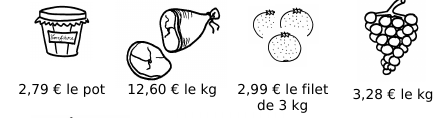
\includegraphics[scale=0.8]{img/IE1-Courses.png} 
\end{minipage}
\begin{minipage}{0.4\textwidth}
J'ai acheté 3 pots de confiture et 2kg de raisin. J'ai payé avec un billet de 20€. Combien de monnaie vais-je récupérer?
\end{minipage}

\vspace{20cm}

\textbf{Exercice Bonus}\\

\begin{minipage}{0.45\textwidth}
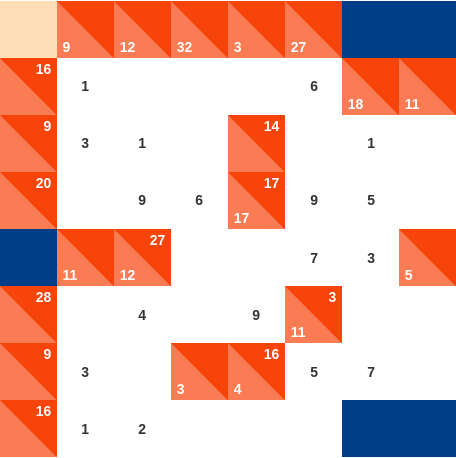
\includegraphics[scale=0.7]{img/IE3-kakuro.png} 
\end{minipage}
\hfill\vline\hfill
\begin{minipage}{0.45\textwidth}
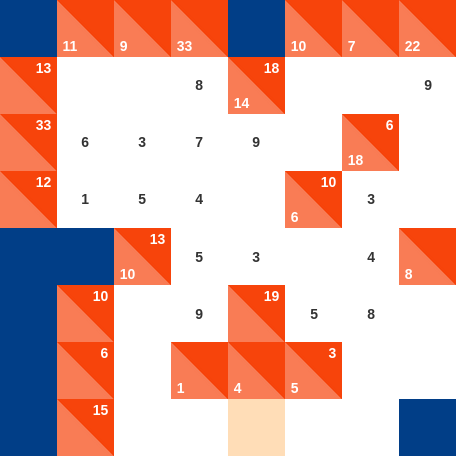
\includegraphics[scale=0.7]{img/IE3-kakuro2.png} 
\end{minipage}

\end{document}